% figures/fig2_access_retention.tex
\begin{figure}[t]
  \centering
  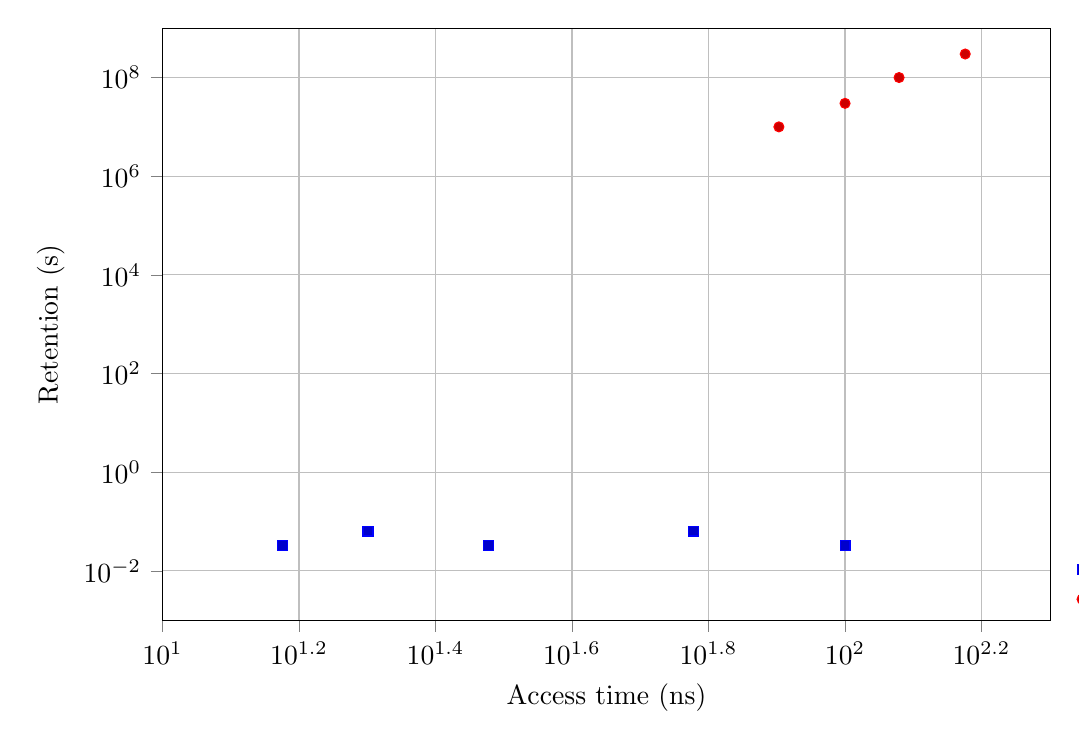
\begin{tikzpicture}
    \begin{loglogaxis}[
      width=0.93\columnwidth,
      height=0.62\columnwidth,
      scale only axis=true,
      xlabel={Access time (ns)},
      ylabel={Retention (s)},
      grid=both,
      tick align=outside,
      tickpos=left,
      xmin=10, xmax=200,
      ymin=1e-3, ymax=1e9,
      xlabel near ticks, ylabel near ticks,
      legend style={
        at={(1.02,0)}, anchor=south west,           % 右外配置
        draw=none, fill=white, font=\scriptsize,
        /tikz/overlay                              % ← バウンディングボックスに含めない
      },
      legend cell align=left
      % clip=false は不要(凡例は overlay で外出し)
    ]

      % LPDDR
      \addplot+[only marks, mark=square*, mark size=1.8pt]
        coordinates {(15,3.2e-2) (20,6.4e-2) (30,3.2e-2) (60,6.4e-2) (100,3.2e-2)};
      \addlegendentry{LPDDR (typ.)}

      % FeRAM
      \addplot+[only marks, mark=*, mark size=1.8pt]
        coordinates {(80,1.0e7) (100,3.0e7) (120,1.0e8) (150,3.0e8)};
      \addlegendentry{FeRAM (typ.)}

    \end{loglogaxis}
  \end{tikzpicture}
  \vspace{-0.6em}
  \caption{Access time vs.\ retention.}
  \label{fig:access_retention_lpddr_feram}
\end{figure}
